\section{Class Diagram cho task assignment module}
    \begin{figure}[h]
        \centering
        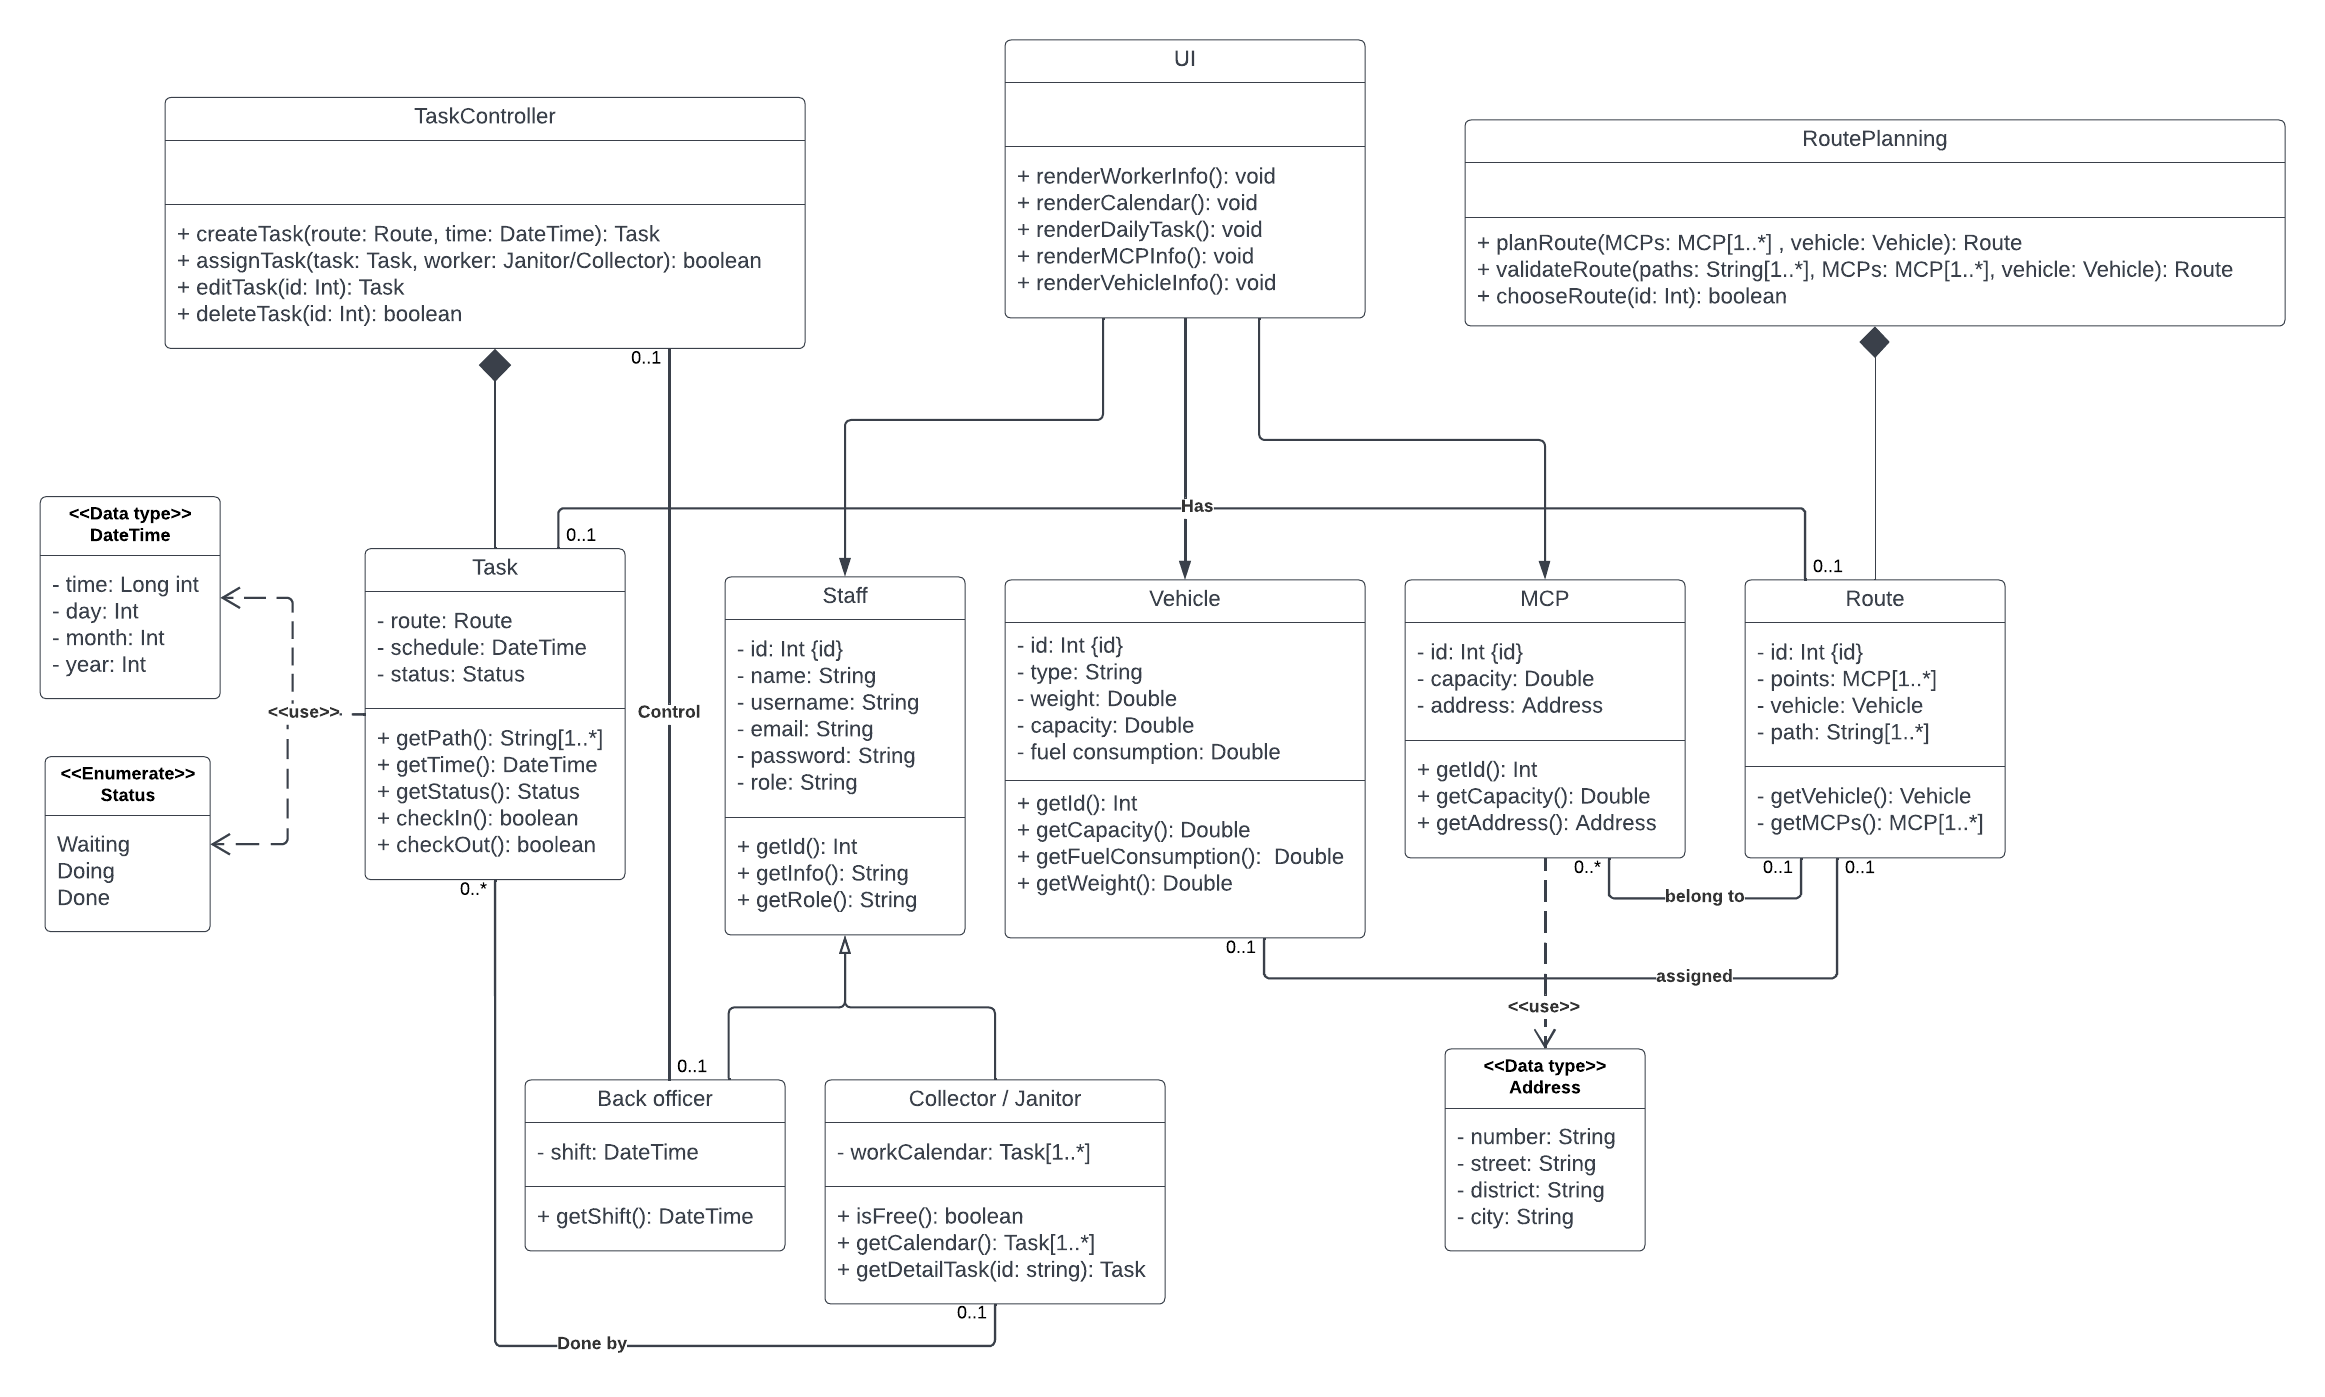
\includegraphics[width=18.0cm,height=15cm]{imgs/class diagram/UWC class diagram.png}
        \caption{Class diagram cho task assignment module}
    \end{figure}
    \newpage
    -Có tất cả 11 class trong module trên gồm có:
    \begin{enumerate}
        \item Class Staff:

        \begin{table}[htp]
            \begin{tabular}{|lll|}
                \hline
                \multicolumn{1}{|l|}{Class Name} & \multicolumn{2}{l|}{Staff}                               \\ \hline
                \multicolumn{1}{|l|}{Inherit}    & \multicolumn{2}{l|}{None}                                \\ \hline
                \multicolumn{3}{|c|}{\cellcolor[HTML]{FFFFC7}Attributes}                                    \\ \hline
                \multicolumn{1}{|l|}{int}        & \multicolumn{1}{l|}{id}        & Số định danh            \\ \hline
                \multicolumn{1}{|l|}{string}     & \multicolumn{1}{l|}{name}      & Tên nhân viên           \\ \hline
                \multicolumn{1}{|l|}{string}     & \multicolumn{1}{l|}{username}  & Tên đăng nhập           \\ \hline
                \multicolumn{1}{|l|}{string}     & \multicolumn{1}{l|}{email}     & Email nhân viên         \\ \hline
                \multicolumn{1}{|l|}{string}     & \multicolumn{1}{l|}{password}  & Mật khẩu                \\ \hline
                \multicolumn{1}{|l|}{string}     & \multicolumn{1}{l|}{role}      & Vai trò                 \\ \hline
                \multicolumn{3}{|c|}{\cellcolor[HTML]{FFFFC7}Methods}                                       \\ \hline
                \multicolumn{1}{|l|}{int}        & \multicolumn{1}{l|}{getId()}   & Lấy số định danh        \\ \hline
                \multicolumn{1}{|l|}{string}     & \multicolumn{1}{l|}{getInfo()} & Lấy thông tin nhân viên \\ \hline
                \multicolumn{1}{|l|}{string}     & \multicolumn{1}{l|}{getRole()} & Lấy thông tin vai trò   \\ \hline
                \multicolumn{3}{|c|}{\cellcolor[HTML]{FFFFC7}Relationships}                                 \\ \hline
            \end{tabular}
        \end{table}
            
        \item Class Collector / Janitor:
    
        \begin{table}[htp]
            \begin{tabular}{|lll|}
                \hline
                \multicolumn{1}{|l|}{Class Name}     & \multicolumn{2}{l|}{Collector/Janitor}                         \\ \hline
                \multicolumn{1}{|l|}{Inherit}        & \multicolumn{2}{l|}{Staff}                                     \\ \hline
                \multicolumn{3}{|c|}{\cellcolor[HTML]{FFFFC7}Attributes}                                              \\ \hline
                \multicolumn{1}{|l|}{Task{[}1..*{]}} & \multicolumn{1}{l|}{workCalendar}    & Lịch làm việc           \\ \hline
                \multicolumn{3}{|c|}{\cellcolor[HTML]{FFFFC7}Methods}                                                 \\ \hline
                \multicolumn{1}{|l|}{boolean}        & \multicolumn{1}{l|}{isFree()}        & Kiểm tra thời gian rảnh \\ \hline
                \multicolumn{1}{|l|}{Task{[}1..*{]}} & \multicolumn{1}{l|}{getCalendar()}   & Lấy lịch làm việc       \\ \hline
                \multicolumn{1}{|l|}{Task}           & \multicolumn{1}{l|}{getDetailTask()} & Lấy task cụ thể         \\ \hline
                \multicolumn{3}{|c|}{\cellcolor[HTML]{FFFFC7}Relationships}                                           \\ \hline
            \end{tabular}
        \end{table}
        
        \item Class Back officer:
        
        \begin{table}[htp]
            \begin{tabular}{|lll|}
                \hline
                \multicolumn{1}{|l|}{Class Name} & \multicolumn{2}{l|}{Back officer}                 \\ \hline
                \multicolumn{1}{|l|}{Inherit}    & \multicolumn{2}{l|}{Staff}                        \\ \hline
                \multicolumn{3}{|c|}{\cellcolor[HTML]{FFFFC7}Attributes}                             \\ \hline
                \multicolumn{1}{|l|}{DateTime}   & \multicolumn{1}{l|}{shift}      & Ca làm việc     \\ \hline
                \multicolumn{3}{|c|}{\cellcolor[HTML]{FFFFC7}Methods}                                \\ \hline
                \multicolumn{1}{|l|}{DateTime}   & \multicolumn{1}{l|}{getShift()} & Lấy ca làm việc \\ \hline
                \multicolumn{3}{|c|}{\cellcolor[HTML]{FFFFC7}Relationships}                          \\ \hline
                \multicolumn{1}{|l|}{control}    & \multicolumn{2}{l|}{Kiểm soát TaskController}     \\ \hline
                \end{tabular}
            \end{table}
        \newpage
        
        \item Class Task:
            
        \begin{table}[htp]
            \begin{tabular}{|lll|}
                \hline
                \multicolumn{1}{|l|}{Class Name}       & \multicolumn{2}{l|}{Task}                                   \\ \hline
                \multicolumn{1}{|l|}{Inherit}          & \multicolumn{2}{l|}{None}                                   \\ \hline
                \multicolumn{3}{|c|}{\cellcolor[HTML]{FFFFC7}Attributes}                                             \\ \hline
                \multicolumn{1}{|l|}{Route}            & \multicolumn{1}{l|}{route}       & Tuyến đường              \\ \hline
                \multicolumn{1}{|l|}{DateTime}         & \multicolumn{1}{l|}{schedule}    & Thời gian làm task       \\ \hline
                \multicolumn{1}{|l|}{Status}           & \multicolumn{1}{l|}{status}      & Trạng thái công việc     \\ \hline
                \multicolumn{3}{|c|}{\cellcolor[HTML]{FFFFC7}Methods}                                                \\ \hline
                \multicolumn{1}{|l|}{string{[}{]}} & \multicolumn{1}{l|}{getPath()}   & Lấy đường đi             \\ \hline
                \multicolumn{1}{|l|}{DateTime}         & \multicolumn{1}{l|}{getTime()}   & Lấy thời gian làm task   \\ \hline
                \multicolumn{1}{|l|}{Status}           & \multicolumn{1}{l|}{getStatus()} & Lấy trạng thái công việc \\ \hline
                \multicolumn{1}{|l|}{boolean}          & \multicolumn{1}{l|}{checkIn()}   & Check in task            \\ \hline
                \multicolumn{1}{|l|}{boolean}          & \multicolumn{1}{l|}{checkOut()}  & Check out task           \\ \hline
                \multicolumn{3}{|c|}{\cellcolor[HTML]{FFFFC7}Relationships}                                          \\ \hline
                \multicolumn{1}{|l|}{Has}              & \multicolumn{2}{l|}{Có chứa Route}                          \\ \hline
                \multicolumn{1}{|l|}{Done by}          & \multicolumn{2}{l|}{Được làm bởi Collector/Janitor}         \\ \hline
            \end{tabular}
        \end{table}
        
        \item Class Vehicle:
    
        \begin{table}[htp]
            \begin{tabular}{|lll|}
                \hline
                \multicolumn{1}{|l|}{Class Name} & \multicolumn{2}{l|}{Vehicle}                                            \\ \hline
                \multicolumn{1}{|l|}{Inherit}    & \multicolumn{2}{l|}{None}                                               \\ \hline
                \multicolumn{3}{|c|}{\cellcolor[HTML]{FFFFC7}Attributes}                                                   \\ \hline
                \multicolumn{1}{|l|}{int}        & \multicolumn{1}{l|}{id}                   & Số định danh                \\ \hline
                \multicolumn{1}{|l|}{string}     & \multicolumn{1}{l|}{type}                 & Loại phương tiện            \\ \hline
                \multicolumn{1}{|l|}{double}     & \multicolumn{1}{l|}{weight}               & Khối lượng phương tiện      \\ \hline
                \multicolumn{1}{|l|}{double}     & \multicolumn{1}{l|}{capacity}             & Sức chứa                    \\ \hline
                \multicolumn{1}{|l|}{double}     & \multicolumn{1}{l|}{fuelConsumption}      & Mức tiêu thụ nhiên liệu     \\ \hline
                \multicolumn{3}{|c|}{\cellcolor[HTML]{FFFFC7}Methods}                                                      \\ \hline
                \multicolumn{1}{|l|}{int}        & \multicolumn{1}{l|}{getId()}              & Lấy số định danh            \\ \hline
                \multicolumn{1}{|l|}{double}     & \multicolumn{1}{l|}{getCapacity()}        & Lấy sức chứa                \\ \hline
                \multicolumn{1}{|l|}{double}     & \multicolumn{1}{l|}{getFuelConsumption()} & Lấy mức tiêu thụ nhiên liệu \\ \hline
                \multicolumn{1}{|l|}{double}     & \multicolumn{1}{l|}{getWeight()}          & Lấy khối lượng              \\ \hline
                \multicolumn{3}{|c|}{\cellcolor[HTML]{FFFFC7}Relationships}                                                \\ \hline
                \multicolumn{1}{|l|}{assigned}   & \multicolumn{2}{l|}{Gán tuyến đường cho phương tiện}                    \\ \hline
            \end{tabular}
        \end{table}
        
        \newpage
        \item Class MCP:
           
        \begin{table}[htp]
            \begin{tabular}{|lll|}
                \hline
                \multicolumn{1}{|l|}{Class Name} & \multicolumn{2}{l|}{MCP}                              \\ \hline
                \multicolumn{1}{|l|}{Inherit}    & \multicolumn{2}{l|}{None}                             \\ \hline
                \multicolumn{3}{|c|}{\cellcolor[HTML]{FFFFC7}Attributes}                                 \\ \hline
                \multicolumn{1}{|l|}{int}        & \multicolumn{1}{l|}{id}            & Số định danh     \\ \hline
                \multicolumn{1}{|l|}{double}     & \multicolumn{1}{l|}{capacity}      & Sức chứa         \\ \hline
                \multicolumn{1}{|l|}{Address}    & \multicolumn{1}{l|}{address}       & Địa chỉ          \\ \hline
                \multicolumn{3}{|c|}{\cellcolor[HTML]{FFFFC7}Methods}                                    \\ \hline
                \multicolumn{1}{|l|}{int}        & \multicolumn{1}{l|}{getId()}       & Lấy số định danh \\ \hline
                \multicolumn{1}{|l|}{double}     & \multicolumn{1}{l|}{getCapacity()} & Lấy sức chứa     \\ \hline
                \multicolumn{1}{|l|}{Address}    & \multicolumn{1}{l|}{getAddress()}  & Lấy địa chỉ      \\ \hline
                \multicolumn{3}{|c|}{\cellcolor[HTML]{FFFFC7}Relationships}                              \\ \hline
                \multicolumn{1}{|l|}{belong to}  & \multicolumn{2}{l|}{MCP thuộc tuyến đường}            \\ \hline
            \end{tabular}
        \end{table}

        \item Class Route:

        \begin{table}[htp]
            \begin{tabular}{|lll|}
                \hline
                \multicolumn{1}{|l|}{Class Name}    & \multicolumn{2}{l|}{Route}                                \\ \hline
                \multicolumn{1}{|l|}{Inherit}       & \multicolumn{2}{l|}{None}                                 \\ \hline
                \multicolumn{3}{|c|}{\cellcolor[HTML]{FFFFC7}Attributes}                                        \\ \hline
                \multicolumn{1}{|l|}{int}           & \multicolumn{1}{l|}{id}           & Số định danh          \\ \hline
                \multicolumn{1}{|l|}{MCP{[}1..*{]}} & \multicolumn{1}{l|}{points}       & Danh sách các MCP     \\ \hline
                \multicolumn{1}{|l|}{Vehicle}       & \multicolumn{1}{l|}{vehicle}      & Phương tiện           \\ \hline
                \multicolumn{1}{|l|}{string}        & \multicolumn{1}{l|}{path}         & Đường đi              \\ \hline
                \multicolumn{3}{|c|}{\cellcolor[HTML]{FFFFC7}Methods}                                           \\ \hline
                \multicolumn{1}{|l|}{Vehicle}       & \multicolumn{1}{l|}{getVehicle()} & Lấy phương tiện       \\ \hline
                \multicolumn{1}{|l|}{MCP{[}1..*{]}} & \multicolumn{1}{l|}{getMCPs}      & Lấy danh sách các MCP \\ \hline
                \multicolumn{3}{|c|}{\cellcolor[HTML]{FFFFC7}Relationships}                                     \\ \hline
            \end{tabular}
        \end{table}

        \newpage
        \item Class RoutePlanning:

        \begin{table}[htp]
            \begin{tabular}{|lll|}
                \hline
                \multicolumn{1}{|l|}{Class Name}  & \multicolumn{2}{l|}{RoutePlanning}                                                                                        \\ \hline
                \multicolumn{1}{|l|}{Inherit}     & \multicolumn{2}{l|}{None}                                                                                                 \\ \hline
                \multicolumn{3}{|c|}{\cellcolor[HTML]{FFFFC7}Attributes}                                                                                                      \\ \hline
                \multicolumn{3}{|c|}{\cellcolor[HTML]{FFFFC7}Methods}                                                                                                         \\ \hline
                \multicolumn{1}{|l|}{Route}       & \multicolumn{1}{l|}{planRoute(MCPs: MCP{[}1..*{]}, vehicle: Vehicle)}                              & Lập tuyến đường      \\ \hline
                \multicolumn{1}{|l|}{Route}       & \multicolumn{1}{l|}{validateRoute(paths: string{[}1..*{]}, MCPs: MCP{[}1..*{]}, vehicle: Vehicle)} & Đánh giá tuyến đường \\ \hline
                \multicolumn{1}{|l|}{boolean}     & \multicolumn{1}{l|}{chooseRoute(id: int)}                                                          & Chọn tuyến đường     \\ \hline
                \multicolumn{1}{|l|}{boolean}     & \multicolumn{1}{l|}{getRoutte(id: int)}                                                            & Lấy tuyến đường      \\ \hline
                \multicolumn{3}{|c|}{\cellcolor[HTML]{FFFFC7}Relationships}                                                                                                   \\ \hline
                \multicolumn{1}{|l|}{Composition} & \multicolumn{2}{l|}{Bao gồm class Route}                                                                                  \\ \hline
            \end{tabular}
        \end{table}

        \item Class TaskController:

        \begin{table}[htp]
            \begin{tabular}{|lll|}
                \hline
                \multicolumn{1}{|l|}{Class Name}  & \multicolumn{2}{l|}{TaskController}                                                                     \\ \hline
                \multicolumn{1}{|l|}{Inherit}     & \multicolumn{2}{l|}{None}                                                                               \\ \hline
                \multicolumn{3}{|c|}{\cellcolor[HTML]{FFFFC7}Attributes}                                                                                    \\ \hline
                \multicolumn{3}{|c|}{\cellcolor[HTML]{FFFFC7}Methods}                                                                                       \\ \hline
                \multicolumn{1}{|l|}{Task}        & \multicolumn{1}{l|}{createTask(route: Route, time: DateTime)}          & Tạo task                       \\ \hline
                \multicolumn{1}{|l|}{boolean}     & \multicolumn{1}{l|}{assignTask(task: Task, worker: Collector/Janitor)} & Gán task cho collector/janitor \\ \hline
                \multicolumn{1}{|l|}{Task}        & \multicolumn{1}{l|}{editTask(id: Int)}                                 & Điều chỉnh task                \\ \hline
                \multicolumn{1}{|l|}{boolean}     & \multicolumn{1}{l|}{deleteTask(id: Int)}                               & Xóa task                       \\ \hline
                \multicolumn{1}{|l|}{boolean}     & \multicolumn{1}{l|}{getTask(id: Int)}                                  & Lấy thông tin task             \\ \hline
                \multicolumn{3}{|c|}{\cellcolor[HTML]{FFFFC7}Relationships}                                                                                 \\ \hline
                \multicolumn{1}{|l|}{Composition} & \multicolumn{2}{l|}{Bao gồm class Task}                                                                 \\ \hline
            \end{tabular}
        \end{table}

        \item Class Task View:

        \begin{table}[htp]
            \begin{tabular}{|lll|}
                \hline
                \multicolumn{1}{|l|}{Class Name} & \multicolumn{2}{l|}{Task View}                                          \\ \hline
                \multicolumn{1}{|l|}{Inherit}    & \multicolumn{2}{l|}{None}                                               \\ \hline
                \multicolumn{3}{|c|}{\cellcolor[HTML]{FFFFC7}Attributes}                                                   \\ \hline
                \multicolumn{3}{|c|}{\cellcolor[HTML]{FFFFC7}Methods}                                                      \\ \hline
                \multicolumn{1}{|l|}{void}       & \multicolumn{1}{l|}{renderWorkCalendar()} & Render lịch làm việc        \\ \hline
                \multicolumn{1}{|l|}{void}       & \multicolumn{1}{l|}{renderDailyTask()}   & Render task hàng ngày        \\ \hline
                \multicolumn{3}{|c|}{\cellcolor[HTML]{FFFFC7}Relationships}                                                \\ \hline
                \multicolumn{1}{|l|}{call}   & \multicolumn{2}{l|}{Yêu cầu controller lấy dữ liệu}                         \\ \hline
                \end{tabular}
            \end{table}

        \newpage
        \item Class Route View:

        \begin{table}[htp]
            \begin{tabular}{|lll|}
                \hline
                \multicolumn{1}{|l|}{Class Name} & \multicolumn{2}{l|}{Route View}                                          \\ \hline
                \multicolumn{1}{|l|}{Inherit}    & \multicolumn{2}{l|}{None}                                               \\ \hline
                \multicolumn{3}{|c|}{\cellcolor[HTML]{FFFFC7}Attributes}                                                   \\ \hline
                \multicolumn{3}{|c|}{\cellcolor[HTML]{FFFFC7}Methods}                                                      \\ \hline
                \multicolumn{1}{|l|}{void}       & \multicolumn{1}{l|}{renderMap()} & Render bản đồ                        \\ \hline
                \multicolumn{1}{|l|}{void}       & \multicolumn{1}{l|}{renderInfo()}   & Render thông tin                  \\ \hline
                \multicolumn{1}{|l|}{void}       & \multicolumn{1}{l|}{renderPathBetweenMCP()}   & Render đường đi giữa các MCP  \\ \hline
                \multicolumn{3}{|c|}{\cellcolor[HTML]{FFFFC7}Relationships}                                                \\ \hline
                \multicolumn{1}{|l|}{call}   & \multicolumn{2}{l|}{Yêu cầu controller lấy dữ liệu}                         \\ \hline
            \end{tabular}
        \end{table}
    \end{enumerate}